% !TEX root = ../main.tex

\section{Problem analysis and design} \label{sec:analysis-design} 

The main challenges are already hinted at in section~\ref{sec:goals}. All these
goals pose different problems. These problems (and especially their solutions)
is best analyzed when also discussing the chosen design.

% ------------------------------------------------------------------------------
% ALGORITHM DESIGN PARADIGM
% ------------------------------------------------------------------------------

\subsection{Genetic Algorithm Design Paradigm: General vs. Specific}
\label{sec:GA-design-paradigm}

A genetic algorithm is a very general tool. In the most simple of cases, the
individuals manipulated are simple solution strings containing 1s and 0s - or
other simple characters. The individual is thus a simple entity, and the value
of it only becomes meaningful in the context of a given problem.

In the context of finding structural break points with the rectangle fitness
method, the genome of the individuals contains two types of alleles: \texttt{0}
meaning no break point and \texttt{1} meaning a break point. Thus, the genome
has $T$ genes, where each gene can contain one of two types of alleles. 

The \textit{general paradigm} is alluring due to its simplicity. This is
especially the case within the biological narrative of the genetic algorithm: A
genome of fixed length and a small set of alleles matches the narrative. But for
this problem, where the number of breakpoints is potentially miniscule compared
to the length of the time series, there is a more efficient approach. The
specific approach.  


\subsubsection{Specific Paradigm: The Optimized Approach}
\label{sec:specific-approach}

The \textit{specific paradigm} is made specifically for the problem at hand. For
detecting structural break points, the biggest modification is this: The genomes
no longer contain genes with non-break-point-alleles. The genome is in stead a
list-structure $G$. At each gene $g$ is an allele $a_g$, $G(g) = a_g = (b_g,
B_g)$. The value $b_g$ is itself an index representing the index of the break
point, $b_g \in [0, T]$. The term $B_g$ is a more abstract value containing
information relevant for the fitness model. 


% ------------------------------------------------------------------------------
% Modified Genetic Algorithm Procedures
% ------------------------------------------------------------------------------

\subsection{Modified Genetic Algorithm Procedures} \label{sec:modified-procedures}

Going from a general approach to a specific approach changes how the
genome-altering procedures work. In the following, each individual will be
represented by only its genome. This
might not be the case for the actual implementation, but it will now serve as a
mean to simplification. The sentence "An individual $I$" will actually mean "An
individual with genome $I$". 

\subsubsection{One Point Crossover} \label{sec:one-point-crossover}

The most simple to adapt is the \texttt{one point crossover procedure}: A random
index $i \in [1, T-1]$ is chosen as the splitting point. From the first parent
$P$, the offspring $O$ gets all genes $p$ with alleles $a_p = (b_p, B_p)$ where
$b_p < i$. From the second parent $Q$, $O$ gets all genes $q$ with alleles $a_q
= (b_q. B_q)$ where $b_q \geq i$. The time complexity is $O(Size(P) + Size(Q))$.

\subsubsection{Mutation} \label{sec:mutation}

The mutation procedure is also simple, or at least \textit{made} simple. A single
index $i$ is randomly selected in the interval $[1, T - 1]$. With a probability
$p_m$ a break point is placed at $i$. Else, with a probability $1 - p_m$, the point will become at
non-break-point. This means that if a break point already exists with index $i$,
the break point is removed. If no break point exists at $i$, then no action is
performed. The time complexity for this mutation is $O(T^{-1})$ which is a lot
better than going through $T$ elements as in the handed out pseudo code. 

For the mutation procedure it might be possible that there exists multiple break
points at one index. This is allowed and in stead affects the fitness score. If
a break point is removed at index with multiple break points, only one of the
break points is removed. 

\todo{Explain the fitness thing somewhere else and link to
that from here}

\subsubsection{Uniform crossover} \label{sec:uniform-crossover}

The final procedure, uniform crossover, is a bit more complex in the new
context. The uniform crossover takes two parents $P$ and $Q$. In a single for
loop, the two genomes are both traversed by maintaining two iteration
parameters. $i$ traversing $P$ and $j$ traversing $Q$. The two parameters are
initialized to $i = j = 1$. The break point indexes at the genes $p_i$ and $q_j$
are compared: The allele storing the lowest break point index is added to the
offspring with a fifty-fifty chance. The iteration parameter for that genome is
incremented. If the two break point indexes are the same, a coin toss decides
which allele is added to the offspring. Both counters are incremented afterward.
This is repeated until both genomes are traversed. The time complexity for this
is $O(Size(P) + Size(Q))$. 

Figure~\ref{fig:uniform-crossover} shows an example. The two parents $P$ and $Q$
have three and two break points in the interval respectively. The diagram
contains four scenarios:

\begin{enumerate}
    \item For $i = j = 1$, the break point index $p_1 < q_1$. Thus, the allele
    storing $p_1$ is added to the offspring with a fifty-fifty chance. Now $i$
    is incremented so $i = 2$ 
    
    \item $q_1 < p_2$. Allele storing $q_1$ is selected and $j$ is incremented
    $j = 2$. 
    
    \item $p_2 < q_2$: Allele storing $p_2$ is selected and $i$ is incremented 
    to $i = 3$. 
    
    \item $p_3 = q_2$: A random allele of the two is selected and both $i$ and
    $j$ are incremented to $i = 4$ and $j = 3$. 
\end{enumerate}


\begin{figure}[h]
    \centering
    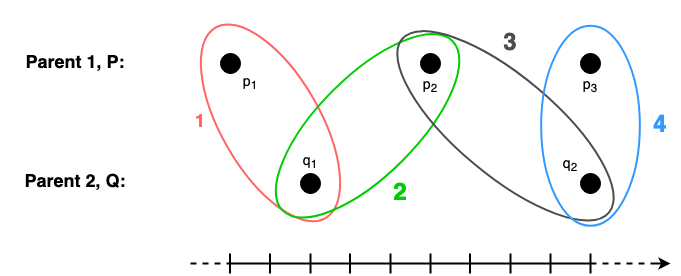
\includegraphics[width=.8\textwidth]{fig/uniform-crossover.png}
    \caption{A diagram showing multiple cases when calculating uniform crossover.}
    \label{fig:uniform-crossover}
\end{figure}


% ------------------------------------------------------------------------------
% Model View Controller
% ------------------------------------------------------------------------------

\subsection{Model-View-Controller}

\subsubsection{Observer pattern}

The observer pattern is not implemented here as the application is very small. A
more simple approach is simply to allow the controller and the business logic to
exchange information. The business logic can, in this application, never change
if no changes are performed in the GUI. This makes observer pattern rather
useless. 

The absence of the observer pattern will result in the controller having direct
access to the business logic. This is not inherently bad and will make the
controller easier to follow. It will possibly result in a bit more cluttered
controller class. But hopefully the simplicity will outweigh potential
negatives. 





